\documentclass[tikz,border=2pt]{standalone}
\usepackage{tikz}
\usepackage{fontspec}
\usepackage{ifthen}
\usetikzlibrary{arrows.meta,positioning,fit,calc,patterns,decorations.pathreplacing}

% Brand colors
\definecolor{Garnet}{HTML}{73000A}
\definecolor{Black90}{HTML}{363636}
\definecolor{Black70}{HTML}{5C5C5C}
\definecolor{Black50}{HTML}{A2A2A2}
\definecolor{Black30}{HTML}{C7C7C7}
\definecolor{Black10}{HTML}{ECECEC}
\definecolor{Rose}{HTML}{CC2E40}
\definecolor{Atlantic}{HTML}{466A9F}
\definecolor{Horseshoe}{HTML}{65780B}
\definecolor{Congaree}{HTML}{1F414D}
\definecolor{WarmGrey}{HTML}{676156}
\definecolor{Sandstorm}{HTML}{FFF2E3}

\newcommand{\pw}{14}
\newcommand{\ph}{9}
\newcommand{\lw}{4.6}
\newcommand{\rs}{5.0}
\newcommand{\tbh}{0.55}
\newcommand{\nbh}{0.38}
\newcommand{\sbh}{0.35}

% ── Reusable macros ──────────────────────────────────────────────

% Top bar
\newcommand{\drawtopbar}{%
  \fill[Garnet] (0,\ph) rectangle (\pw,\ph-\tbh);
  \node[anchor=west,text=white,font=\bfseries\fontsize{7}{8}\selectfont] at (0.15,\ph-0.275) {UOFSC COURSE SCHEDULER};
  % Term selector
  \draw[white,thin] (\pw-1.6,\ph-0.12) rectangle (\pw-0.15,\ph-0.43);
  \node[font=\fontsize{4.5}{5}\selectfont,text=white,anchor=west] at (\pw-1.55,\ph-0.175) {\textsc{term}};
  \fill[white] (\pw-1.3,\ph-0.15) rectangle (\pw-0.2,\ph-0.41);
  \node[font=\fontsize{4.5}{5}\selectfont,text=Black90] at (\pw-0.75,\ph-0.28) {Fall 2026};
}

% Nav bar
\newcommand{\drawnavbar}[1]{%
  \fill[Black90] (0,\ph-\tbh) rectangle (\pw,\ph-\tbh-\nbh);
  \foreach \name/\xpos in {Home/0.5, Degree Plan/1.65, Browse/2.95, Schedule/3.95, Profile/4.9, Export/5.7} {
    \ifthenelse{\equal{\name}{#1}}{%
      \fill[white] (\xpos-0.4,\ph-\tbh) rectangle (\xpos+0.4,\ph-\tbh-\nbh);
      \node[font=\fontsize{4.5}{5}\selectfont,text=Black90] at (\xpos,\ph-\tbh-0.19) {\name};
    }{%
      \node[font=\fontsize{4.5}{5}\selectfont,text=Black30] at (\xpos,\ph-\tbh-0.19) {\name};
    }
  }
}

% Status bar
\newcommand{\drawstatusbar}[1]{%
  \fill[Black10] (0,0) rectangle (\pw,\sbh);
  \draw[Black30] (0,\sbh) -- (\pw,\sbh);
  \node[font=\fontsize{4}{5}\selectfont,text=Black70,anchor=west] at (0.15,0.175) {#1};
}

% Left panel background
\newcommand{\drawleftpanel}{%
  \pgfmathsetmacro{\paneltop}{\ph-\tbh-\nbh}
  \fill[Black10!50!white] (0,\sbh) rectangle (\lw,\paneltop);
  \draw[Black30] (\lw,\sbh) -- (\lw,\paneltop);
}

% Schedule grid
\newcommand{\drawschedulegrid}{%
  \pgfmathsetmacro{\gridtop}{\ph-\tbh-\nbh-0.1}
  \pgfmathsetmacro{\gridbot}{\sbh+0.1}
  \pgfmathsetmacro{\gridleft}{\rs+0.05}
  \pgfmathsetmacro{\gridright}{\pw-0.1}
  \pgfmathsetmacro{\timelabelx}{\gridleft+0.35}
  \pgfmathsetmacro{\colstart}{\gridleft+0.6}
  \pgfmathsetmacro{\colwidth}{(\gridright-\colstart)/5}
  % Header row
  \fill[Garnet] (\colstart,\gridtop) rectangle (\gridright,\gridtop-0.3);
  \foreach \day/\idx in {MON/0,TUE/1,WED/2,THU/3,FRI/4} {
    \pgfmathsetmacro{\cx}{\colstart+\colwidth*\idx+\colwidth/2}
    \node[font=\fontsize{3.8}{4}\selectfont\bfseries,text=white] at (\cx,\gridtop-0.15) {\day};
  }
  % Time labels and grid lines
  \pgfmathsetmacro{\bodyTop}{\gridtop-0.3}
  \pgfmathsetmacro{\bodyHeight}{\bodyTop-\gridbot}
  \foreach \hr/\idx in {8am/0,9am/1,10am/2,11am/3,12pm/4,1pm/5,2pm/6,3pm/7,4pm/8,5pm/9} {
    \pgfmathsetmacro{\yy}{\bodyTop-\bodyHeight*\idx/10}
    \draw[Black30!60!white,very thin] (\colstart,\yy) -- (\gridright,\yy);
    \node[font=\fontsize{2.8}{3}\selectfont,text=Black50,anchor=east] at (\colstart-0.04,\yy) {\hr};
  }
  % Vertical column separators
  \foreach \idx in {1,...,4} {
    \pgfmathsetmacro{\xx}{\colstart+\colwidth*\idx}
    \draw[Black30!60!white,very thin] (\xx,\bodyTop) -- (\xx,\gridbot);
  }
  % Outer border
  \draw[Black30] (\gridleft,\gridtop) rectangle (\gridright,\gridbot);
}

% Helper: draw a course block on the schedule
% #1=day index (0-4), #2=start hour (decimal from 8), #3=end hour, #4=color, #5=label, #6=style(solid/dashed)
\newcommand{\drawcourseblock}[6]{%
  \pgfmathsetmacro{\gridtop}{\ph-\tbh-\nbh-0.1}
  \pgfmathsetmacro{\gridbot}{\sbh+0.1}
  \pgfmathsetmacro{\colstart}{\rs+0.05+0.6}
  \pgfmathsetmacro{\gridright}{\pw-0.1}
  \pgfmathsetmacro{\colwidth}{(\gridright-\colstart)/5}
  \pgfmathsetmacro{\bodyTop}{\gridtop-0.3}
  \pgfmathsetmacro{\bodyHeight}{\bodyTop-\gridbot}
  \pgfmathsetmacro{\blocktop}{\bodyTop-\bodyHeight*(#2)/10}
  \pgfmathsetmacro{\blockbot}{\bodyTop-\bodyHeight*(#3)/10}
  \pgfmathsetmacro{\blockleft}{\colstart+\colwidth*(#1)+0.04}
  \pgfmathsetmacro{\blockright}{\colstart+\colwidth*(#1)+\colwidth-0.04}
  \ifthenelse{\equal{#6}{dashed}}{%
    \fill[#4!15!white] (\blockleft,\blocktop) rectangle (\blockright,\blockbot);
    \draw[#4,thick,dashed] (\blockleft,\blocktop) rectangle (\blockright,\blockbot);
    \node[font=\fontsize{2.8}{3.2}\selectfont,text=#4,align=center] at ({(\blockleft+\blockright)/2},{(\blocktop+\blockbot)/2}) {#5};
  }{%
    \fill[#4] (\blockleft,\blocktop) rectangle (\blockright,\blockbot);
    \node[font=\fontsize{2.8}{3.2}\selectfont,text=white,align=center] at ({(\blockleft+\blockright)/2},{(\blocktop+\blockbot)/2}) {#5};
  }
}

% Search bar
% #1=placeholder/typed text, #2=y position of top
\newcommand{\drawsearchbar}[2]{%
  \fill[white] (0.15,#2) rectangle (\lw-0.15,#2-0.4);
  \draw[Black30] (0.15,#2) rectangle (\lw-0.15,#2-0.4);
  \node[font=\fontsize{3.5}{4}\selectfont,text=Black50,anchor=west] at (0.25,#2-0.2) {#1};
  \fill[Garnet] (0.15,#2-0.48) rectangle (\lw-0.15,#2-0.78);
  \node[font=\fontsize{4}{5}\selectfont\bfseries,text=white] at ({\lw/2},#2-0.63) {SEARCH COURSES};
}

\begin{document}

%% ═══════════════════════════════════════════════════════════════
%% PAGE 1: Empty State — Ready to Search
%% ═══════════════════════════════════════════════════════════════
\begin{tikzpicture}
  % Stage label
  \node[font=\fontsize{5.5}{6}\selectfont\bfseries,text=Black90,anchor=south west] at (0,\ph+0.15) {Stage 1: Empty State — Ready to Search};

  % Frame
  \draw[Black90,thin] (0,0) rectangle (\pw,\ph);
  \fill[white] (0,0) rectangle (\pw,\ph);

  \drawtopbar
  \drawnavbar{Browse}
  \drawstatusbar{0 courses \,·\, 0 credits \,·\, No conflicts}
  \drawleftpanel
  \drawschedulegrid

  % Left panel content
  \pgfmathsetmacro{\contenttop}{\ph-\tbh-\nbh-0.15}

  % Section header
  \node[font=\fontsize{4.5}{5}\selectfont\bfseries,text=Garnet,anchor=north west] at (0.15,\contenttop) {FIND COURSES};

  % Search bar
  \pgfmathsetmacro{\searchY}{\contenttop-0.35}
  \fill[white] (0.15,\searchY) rectangle (\lw-0.15,\searchY-0.42);
  \draw[Black30] (0.15,\searchY) rectangle (\lw-0.15,\searchY-0.42);
  \node[font=\fontsize{3}{3.5}\selectfont,text=Black50,anchor=west,text width=4cm] at (0.25,\searchY-0.21) {Search: EMCH 508, finite element, Deng, CRN...};

  % Search button
  \pgfmathsetmacro{\btnY}{\searchY-0.52}
  \fill[Garnet] (0.15,\btnY) rectangle (\lw-0.15,\btnY-0.33);
  \node[font=\fontsize{3.8}{4}\selectfont\bfseries,text=white] at ({\lw/2},\btnY-0.165) {SEARCH COURSES};

  % Browse by requirement
  \pgfmathsetmacro{\browseY}{\btnY-0.52}
  \node[font=\fontsize{3.8}{4}\selectfont\bfseries,text=Black70,anchor=north west] at (0.15,\browseY) {Or browse by requirement:};

  % Chips
  \pgfmathsetmacro{\chipY}{\browseY-0.32}
  \foreach \label/\xoff/\w in {Degree Requirements/0/1.45, Gen Ed/1.55/0.7, Minor: Math/2.35/0.95} {
    \fill[white] (0.15+\xoff,\chipY) rectangle (0.15+\xoff+\w,\chipY-0.28);
    \draw[Black30] (0.15+\xoff,\chipY) rectangle (0.15+\xoff+\w,\chipY-0.28);
    \node[font=\fontsize{3}{3.5}\selectfont,text=Black70] at (0.15+\xoff+\w/2,\chipY-0.14) {\label};
  }
  \pgfmathsetmacro{\chipY2}{\chipY-0.38}
  \foreach \label/\xoff/\w in {Concentration/0/1.05, 2nd Major/1.15/0.85} {
    \fill[white] (0.15+\xoff,\chipY2) rectangle (0.15+\xoff+\w,\chipY2-0.28);
    \draw[Black30] (0.15+\xoff,\chipY2) rectangle (0.15+\xoff+\w,\chipY2-0.28);
    \node[font=\fontsize{3}{3.5}\selectfont,text=Black70] at (0.15+\xoff+\w/2,\chipY2-0.14) {\label};
  }

  % Recent courses
  \pgfmathsetmacro{\recentY}{\chipY2-0.55}
  \node[font=\fontsize{3.8}{4}\selectfont\bfseries,text=Black70,anchor=north west] at (0.15,\recentY) {Recent Courses};
  \draw[Black30] (0.15,\recentY-0.08) -- (\lw-0.15,\recentY-0.08);
  \node[font=\fontsize{3}{3.5}\selectfont,text=Black50,anchor=north west,text width=4cm] at (0.15,\recentY-0.2) {No recently viewed courses.};

  % Empty schedule label
  \pgfmathsetmacro{\gridCenterX}{(\rs+\pw)/2}
  \pgfmathsetmacro{\gridCenterY}{(\ph-\tbh-\nbh+\sbh)/2}
  \node[font=\fontsize{4}{5}\selectfont,text=Black30] at (\gridCenterX,\gridCenterY) {Add courses to build your schedule};
\end{tikzpicture}

\newpage
%% ═══════════════════════════════════════════════════════════════
%% PAGE 2: Quick Add — Known Courses
%% ═══════════════════════════════════════════════════════════════
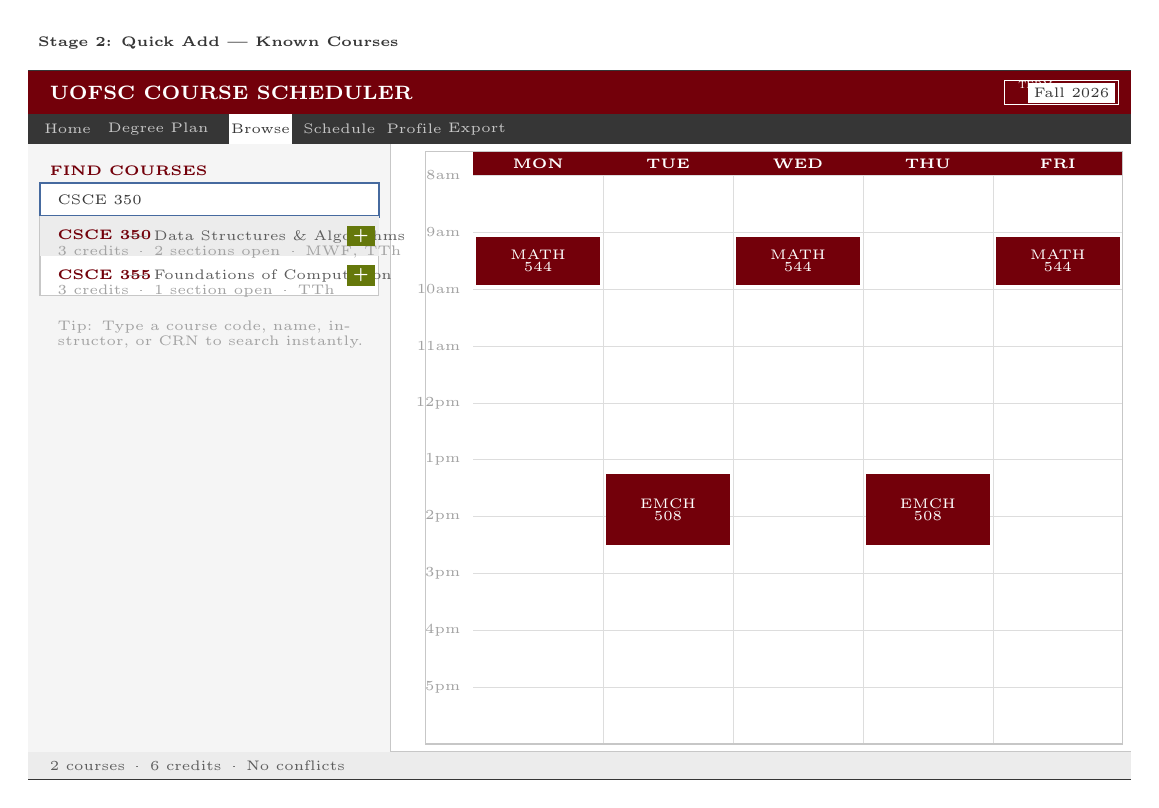
\begin{tikzpicture}
  \node[font=\fontsize{5.5}{6}\selectfont\bfseries,text=Black90,anchor=south west] at (0,\ph+0.15) {Stage 2: Quick Add — Known Courses};

  \draw[Black90,thin] (0,0) rectangle (\pw,\ph);
  \fill[white] (0,0) rectangle (\pw,\ph);

  \drawtopbar
  \drawnavbar{Browse}
  \drawstatusbar{2 courses \,·\, 6 credits \,·\, No conflicts}
  \drawleftpanel
  \drawschedulegrid

  % Left panel
  \pgfmathsetmacro{\contenttop}{\ph-\tbh-\nbh-0.15}
  \node[font=\fontsize{4.5}{5}\selectfont\bfseries,text=Garnet,anchor=north west] at (0.15,\contenttop) {FIND COURSES};

  % Search bar with typed text
  \pgfmathsetmacro{\searchY}{\contenttop-0.35}
  \fill[white] (0.15,\searchY) rectangle (\lw-0.15,\searchY-0.42);
  \draw[Atlantic,thick] (0.15,\searchY) rectangle (\lw-0.15,\searchY-0.42);
  \node[font=\fontsize{3.5}{4}\selectfont,text=Black90,anchor=west] at (0.25,\searchY-0.21) {CSCE 350};

  % Autocomplete dropdown
  \pgfmathsetmacro{\ddY}{\searchY-0.42}
  \fill[white] (0.15,\ddY) rectangle (\lw-0.15,\ddY-1.0);
  \draw[Black30] (0.15,\ddY) rectangle (\lw-0.15,\ddY-1.0);

  % Result row 1 — highlighted
  \fill[Black10] (0.15,\ddY) rectangle (\lw-0.15,\ddY-0.5);
  \node[font=\fontsize{3.5}{4}\selectfont\bfseries,text=Garnet,anchor=north west] at (0.25,\ddY-0.05) {CSCE 350};
  \node[font=\fontsize{3}{3.5}\selectfont,text=Black70,anchor=north west] at (1.15,\ddY-0.06) {— Data Structures \& Algorithms};
  \node[font=\fontsize{2.8}{3}\selectfont,text=Black50,anchor=north west] at (0.25,\ddY-0.25) {3 credits \,·\, 2 sections open \,·\, MWF, TTh};
  % + button
  \fill[Horseshoe] (\lw-0.55,\ddY-0.12) rectangle (\lw-0.2,\ddY-0.38);
  \node[font=\fontsize{5}{6}\selectfont\bfseries,text=white] at (\lw-0.375,\ddY-0.25) {+};

  % Result row 2
  \node[font=\fontsize{3.5}{4}\selectfont\bfseries,text=Garnet,anchor=north west] at (0.25,\ddY-0.55) {CSCE 355};
  \node[font=\fontsize{3}{3.5}\selectfont,text=Black70,anchor=north west] at (1.15,\ddY-0.56) {— Foundations of Computation};
  \node[font=\fontsize{2.8}{3}\selectfont,text=Black50,anchor=north west] at (0.25,\ddY-0.75) {3 credits \,·\, 1 section open \,·\, TTh};
  \fill[Horseshoe] (\lw-0.55,\ddY-0.62) rectangle (\lw-0.2,\ddY-0.88);
  \node[font=\fontsize{5}{6}\selectfont\bfseries,text=white] at (\lw-0.375,\ddY-0.75) {+};

  % Schedule blocks — EMCH 508 TTh 1:15-2:30 (hours 5.25-6.5 from 8am)
  \drawcourseblock{1}{5.25}{6.5}{Garnet}{EMCH\\508}{solid}
  \drawcourseblock{3}{5.25}{6.5}{Garnet}{EMCH\\508}{solid}
  % MATH 544 MWF 9:05-9:55 (hours 1.08-1.92)
  \drawcourseblock{0}{1.08}{1.92}{Garnet}{MATH\\544}{solid}
  \drawcourseblock{2}{1.08}{1.92}{Garnet}{MATH\\544}{solid}
  \drawcourseblock{4}{1.08}{1.92}{Garnet}{MATH\\544}{solid}

  % Helpful hint
  \pgfmathsetmacro{\hintY}{\ddY-1.2}
  \node[font=\fontsize{3}{3.5}\selectfont,text=Black50,anchor=north west,text width=4cm] at (0.25,\hintY) {Tip: Type a course code, name, instructor, or CRN to search instantly.};
\end{tikzpicture}

\newpage
%% ═══════════════════════════════════════════════════════════════
%% PAGE 3: Exploration Mode — Browse by Requirement
%% ═══════════════════════════════════════════════════════════════
\begin{tikzpicture}
  \node[font=\fontsize{5.5}{6}\selectfont\bfseries,text=Black90,anchor=south west] at (0,\ph+0.15) {Stage 3: Exploration Mode — Browse by Requirement};

  \draw[Black90,thin] (0,0) rectangle (\pw,\ph);
  \fill[white] (0,0) rectangle (\pw,\ph);

  \drawtopbar
  \drawnavbar{Browse}
  \drawstatusbar{3 courses \,·\, 9 credits \,·\, No conflicts}
  \drawleftpanel
  \drawschedulegrid

  % Left panel
  \pgfmathsetmacro{\contenttop}{\ph-\tbh-\nbh-0.12}

  % Breadcrumb
  \node[font=\fontsize{3}{3.5}\selectfont,text=Atlantic,anchor=north west] at (0.15,\contenttop) {Requirements > Minor: Mathematics > Elective (pick 2)};

  % Section header
  \pgfmathsetmacro{\secY}{\contenttop-0.28}
  \node[font=\fontsize{4.5}{5}\selectfont\bfseries,text=Garnet,anchor=north west] at (0.15,\secY) {Math Minor Electives};
  \draw[Garnet,thick] (0.15,\secY-0.18) -- (\lw-0.15,\secY-0.18);

  % Filter chips
  \pgfmathsetmacro{\filterY}{\secY-0.38}
  \foreach \label/\xoff/\w in {Open seats/0/0.82, No conflicts/0.9/0.92, Prereqs met/1.9/0.9} {
    \fill[Horseshoe!15!white] (0.15+\xoff,\filterY) rectangle (0.15+\xoff+\w,\filterY-0.24);
    \draw[Horseshoe] (0.15+\xoff,\filterY) rectangle (0.15+\xoff+\w,\filterY-0.24);
    \node[font=\fontsize{2.8}{3}\selectfont,text=Horseshoe] at (0.15+\xoff+\w/2,\filterY-0.12) {\checkmark\;\label};
  }

  % Results header
  \pgfmathsetmacro{\resY}{\filterY-0.42}
  \node[font=\fontsize{3.5}{4}\selectfont,text=Black70,anchor=north west] at (0.15,\resY) {6 courses match \,·\, 4 you can take};

  % Course cards
  \pgfmathsetmacro{\cardY}{\resY-0.22}
  \pgfmathsetmacro{\cardH}{0.72}

  % Card 1 — MATH 546
  \fill[white] (0.15,\cardY) rectangle (\lw-0.15,\cardY-\cardH);
  \draw[Black30] (0.15,\cardY) rectangle (\lw-0.15,\cardY-\cardH);
  \node[font=\fontsize{3.5}{4}\selectfont\bfseries,text=Garnet,anchor=north west] at (0.25,\cardY-0.05) {MATH 546};
  \node[font=\fontsize{3}{3.5}\selectfont,text=Black90,anchor=north west] at (1.1,\cardY-0.06) {Algebraic Structures I};
  \node[font=\fontsize{2.8}{3}\selectfont,text=Black70,anchor=north west] at (0.25,\cardY-0.26) {3 cr \,·\, 1 section \,·\, 15 seats \,·\, MWF 11:15};
  \node[font=\fontsize{2.5}{3}\selectfont,text=Horseshoe,anchor=north west] at (0.25,\cardY-0.43) {Offered: Fall only (last: Fa25)};
  \node[font=\fontsize{2.5}{3}\selectfont,text=Black50,anchor=north west] at (0.25,\cardY-0.56) {Instructor: Johnson};
  % + button
  \fill[Horseshoe] (\lw-0.55,\cardY-0.17) rectangle (\lw-0.2,\cardY-0.43);
  \node[font=\fontsize{5}{6}\selectfont\bfseries,text=white] at (\lw-0.375,\cardY-0.3) {+};

  % Card 2 — MATH 554
  \pgfmathsetmacro{\card_ii}{\cardY-\cardH-0.08}
  \fill[white] (0.15,\card_ii) rectangle (\lw-0.15,\card_ii-\cardH);
  \draw[Black30] (0.15,\card_ii) rectangle (\lw-0.15,\card_ii-\cardH);
  \node[font=\fontsize{3.5}{4}\selectfont\bfseries,text=Garnet,anchor=north west] at (0.25,\card_ii-0.05) {MATH 554};
  \node[font=\fontsize{3}{3.5}\selectfont,text=Black90,anchor=north west] at (1.1,\card_ii-0.06) {Analysis I};
  \node[font=\fontsize{2.8}{3}\selectfont,text=Black70,anchor=north west] at (0.25,\card_ii-0.26) {3 cr \,·\, 2 sections \,·\, 8 seats \,·\, TTh 2:50};
  \node[font=\fontsize{2.5}{3}\selectfont,text=Atlantic,anchor=north west] at (0.25,\card_ii-0.43) {Offered: Every semester};
  \node[font=\fontsize{2.5}{3}\selectfont,text=Black50,anchor=north west] at (0.25,\card_ii-0.56) {Instructor: Williams};
  \fill[Horseshoe] (\lw-0.55,\card_ii-0.17) rectangle (\lw-0.2,\card_ii-0.43);
  \node[font=\fontsize{5}{6}\selectfont\bfseries,text=white] at (\lw-0.375,\card_ii-0.3) {+};

  % Card 3 — MATH 561 (grayed — prereqs not met)
  \pgfmathsetmacro{\card_iii}{\card_ii-\cardH-0.08}
  \fill[Black10] (0.15,\card_iii) rectangle (\lw-0.15,\card_iii-\cardH);
  \draw[Black30] (0.15,\card_iii) rectangle (\lw-0.15,\card_iii-\cardH);
  \node[font=\fontsize{3.5}{4}\selectfont\bfseries,text=Black50,anchor=north west] at (0.25,\card_iii-0.05) {MATH 561};
  \node[font=\fontsize{3}{3.5}\selectfont,text=Black50,anchor=north west] at (1.1,\card_iii-0.06) {Intro Topology};
  \node[font=\fontsize{2.8}{3}\selectfont,text=Black50,anchor=north west] at (0.25,\card_iii-0.26) {3 cr \,·\, 1 section \,·\, 20 seats \,·\, MWF 1:10};
  \node[font=\fontsize{2.5}{3}\selectfont,text=Rose,anchor=north west] at (0.25,\card_iii-0.43) {Missing prereq: MATH 554};
  \node[font=\fontsize{2.5}{3}\selectfont,text=Black50,anchor=north west] at (0.25,\card_iii-0.56) {Offered: Fall only (last: Fa25)};

  % Card 4 — partial, scrollable
  \pgfmathsetmacro{\card_iv}{\card_iii-\cardH-0.08}
  \fill[white] (0.15,\card_iv) rectangle (\lw-0.15,\card_iv-0.35);
  \draw[Black30] (0.15,\card_iv) rectangle (\lw-0.15,\card_iv-0.35);
  \node[font=\fontsize{3.5}{4}\selectfont\bfseries,text=Garnet,anchor=north west] at (0.25,\card_iv-0.05) {MATH 570};
  \node[font=\fontsize{3}{3.5}\selectfont,text=Black90,anchor=north west] at (1.1,\card_iv-0.06) {Discrete Optimization};
  % Scroll indicator
  \node[font=\fontsize{3}{3.5}\selectfont,text=Black50] at ({\lw/2},\card_iv-0.45) {$\downarrow$ scroll for more};

  % Schedule blocks — 3 courses added
  % EMCH 508 TTh 1:15-2:30
  \drawcourseblock{1}{5.25}{6.5}{Garnet}{EMCH\\508}{solid}
  \drawcourseblock{3}{5.25}{6.5}{Garnet}{EMCH\\508}{solid}
  % MATH 544 MWF 9:05-9:55
  \drawcourseblock{0}{1.08}{1.92}{Garnet}{MATH\\544}{solid}
  \drawcourseblock{2}{1.08}{1.92}{Garnet}{MATH\\544}{solid}
  \drawcourseblock{4}{1.08}{1.92}{Garnet}{MATH\\544}{solid}
  % CSCE 350 TTh 10:05-11:20 (hours 2.08-3.33)
  \drawcourseblock{1}{2.08}{3.33}{Garnet}{CSCE\\350}{solid}
  \drawcourseblock{3}{2.08}{3.33}{Garnet}{CSCE\\350}{solid}
\end{tikzpicture}

\newpage
%% ═══════════════════════════════════════════════════════════════
%% PAGE 4: Course Deep Dive — Inline Detail (History Tab)
%% ═══════════════════════════════════════════════════════════════
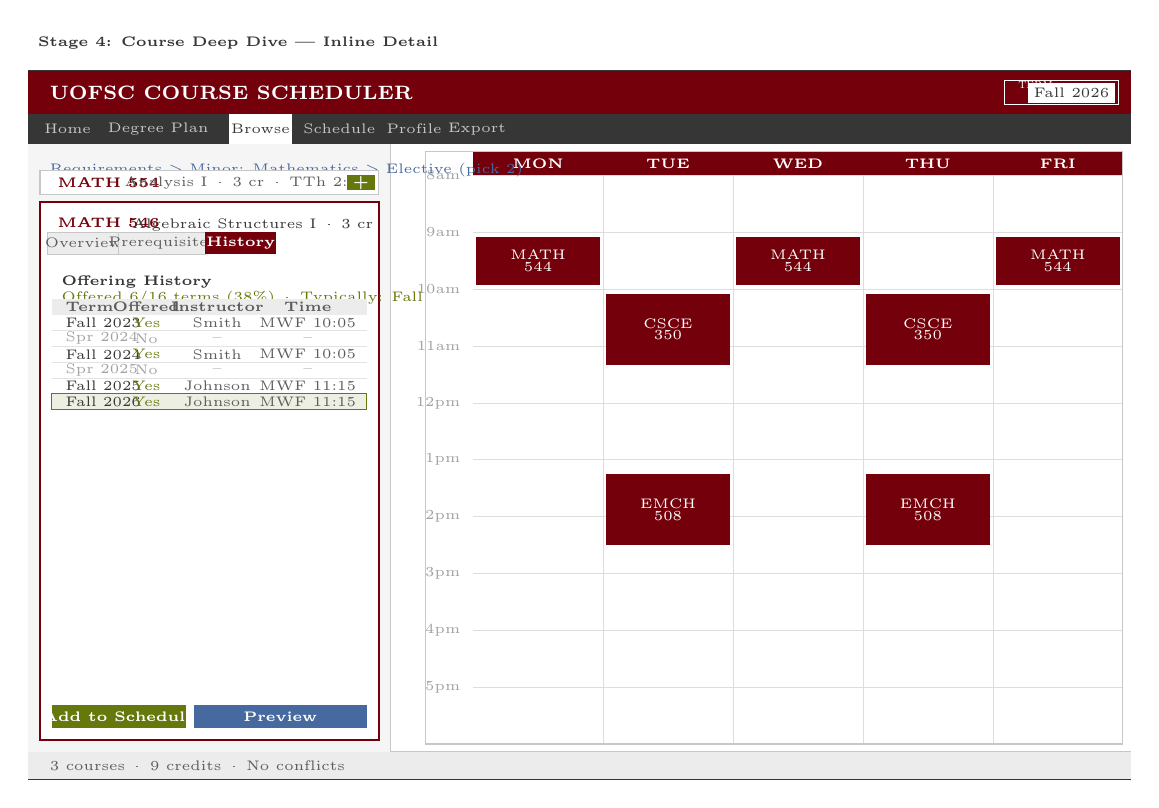
\begin{tikzpicture}
  \node[font=\fontsize{5.5}{6}\selectfont\bfseries,text=Black90,anchor=south west] at (0,\ph+0.15) {Stage 4: Course Deep Dive — Inline Detail};

  \draw[Black90,thin] (0,0) rectangle (\pw,\ph);
  \fill[white] (0,0) rectangle (\pw,\ph);

  \drawtopbar
  \drawnavbar{Browse}
  \drawstatusbar{3 courses \,·\, 9 credits \,·\, No conflicts}
  \drawleftpanel
  \drawschedulegrid

  \pgfmathsetmacro{\contenttop}{\ph-\tbh-\nbh-0.12}

  % Breadcrumb
  \node[font=\fontsize{3}{3.5}\selectfont,text=Atlantic,anchor=north west] at (0.15,\contenttop) {Requirements > Minor: Mathematics > Elective (pick 2)};

  % Compressed card above — MATH 554
  \pgfmathsetmacro{\compY}{\contenttop-0.22}
  \fill[white] (0.15,\compY) rectangle (\lw-0.15,\compY-0.3);
  \draw[Black30] (0.15,\compY) rectangle (\lw-0.15,\compY-0.3);
  \node[font=\fontsize{3}{3.5}\selectfont\bfseries,text=Garnet,anchor=west] at (0.25,\compY-0.15) {MATH 554};
  \node[font=\fontsize{2.8}{3}\selectfont,text=Black70,anchor=west] at (1.1,\compY-0.15) {Analysis I \,·\, 3 cr \,·\, TTh 2:50};
  \fill[Horseshoe] (\lw-0.55,\compY-0.05) rectangle (\lw-0.2,\compY-0.25);
  \node[font=\fontsize{4}{5}\selectfont\bfseries,text=white] at (\lw-0.375,\compY-0.15) {+};

  % ── EXPANDED DETAIL CARD: MATH 546 ──
  \pgfmathsetmacro{\expTop}{\compY-0.4}
  \pgfmathsetmacro{\expBot}{\sbh+0.15}
  \fill[white] (0.15,\expTop) rectangle (\lw-0.15,\expBot);
  \draw[Garnet,thick] (0.15,\expTop) rectangle (\lw-0.15,\expBot);

  % Course title
  \node[font=\fontsize{4}{5}\selectfont\bfseries,text=Garnet,anchor=north west] at (0.25,\expTop-0.08) {MATH 546};
  \node[font=\fontsize{3.2}{4}\selectfont,text=Black90,anchor=north west] at (1.2,\expTop-0.09) {Algebraic Structures I \,·\, 3 cr};

  % Tabs
  \pgfmathsetmacro{\tabY}{\expTop-0.38}
  \pgfmathsetmacro{\tabH}{0.28}
  % Overview tab (inactive)
  \fill[Black10] (0.25,\tabY) rectangle (1.15,\tabY-\tabH);
  \draw[Black30] (0.25,\tabY) rectangle (1.15,\tabY-\tabH);
  \node[font=\fontsize{3}{3.5}\selectfont,text=Black70] at (0.7,\tabY-0.14) {Overview};
  % Prerequisites tab (inactive)
  \fill[Black10] (1.15,\tabY) rectangle (2.25,\tabY-\tabH);
  \draw[Black30] (1.15,\tabY) rectangle (2.25,\tabY-\tabH);
  \node[font=\fontsize{3}{3.5}\selectfont,text=Black70] at (1.7,\tabY-0.14) {Prerequisites};
  % History tab (active)
  \fill[Garnet] (2.25,\tabY) rectangle (3.15,\tabY-\tabH);
  \node[font=\fontsize{3}{3.5}\selectfont\bfseries,text=white] at (2.7,\tabY-0.14) {History};

  % History content
  \pgfmathsetmacro{\histY}{\tabY-\tabH-0.15}
  \node[font=\fontsize{3.5}{4}\selectfont\bfseries,text=Black90,anchor=north west] at (0.3,\histY) {Offering History};
  \pgfmathsetmacro{\statsY}{\histY-0.2}
  \node[font=\fontsize{2.8}{3}\selectfont,text=Horseshoe,anchor=north west] at (0.3,\statsY) {Offered 6/16 terms (38\%) \,·\, Typically: Fall};

  % Table header
  \pgfmathsetmacro{\tblY}{\statsY-0.22}
  \fill[Black10] (0.3,\tblY) rectangle (\lw-0.3,\tblY-0.2);
  \node[font=\fontsize{2.5}{3}\selectfont\bfseries,text=Black70,anchor=west] at (0.35,\tblY-0.1) {Term};
  \node[font=\fontsize{2.5}{3}\selectfont\bfseries,text=Black70] at (1.5,\tblY-0.1) {Offered};
  \node[font=\fontsize{2.5}{3}\selectfont\bfseries,text=Black70] at (2.4,\tblY-0.1) {Instructor};
  \node[font=\fontsize{2.5}{3}\selectfont\bfseries,text=Black70] at (3.55,\tblY-0.1) {Time};

  % Table rows
  \pgfmathsetmacro{\rowH}{0.2}
  \foreach \term/\offered/\inst/\time/\idx/\highlight in {
    Fall 2023/Yes/Smith/MWF 10:05/0/0,
    Spr 2024/No/-/-/1/0,
    Fall 2024/Yes/Smith/MWF 10:05/2/0,
    Spr 2025/No/-/-/3/0,
    Fall 2025/Yes/Johnson/MWF 11:15/4/0,
    Fall 2026/Yes/Johnson/MWF 11:15/5/1%
  } {
    \pgfmathsetmacro{\ry}{\tblY-0.2-\rowH*\idx}
    \ifthenelse{\equal{\highlight}{1}}{%
      \fill[Horseshoe!12!white] (0.3,\ry) rectangle (\lw-0.3,\ry-\rowH);
      \draw[Horseshoe,thin] (0.3,\ry) rectangle (\lw-0.3,\ry-\rowH);
    }{%
      \draw[Black30!50!white,very thin] (0.3,\ry-\rowH) -- (\lw-0.3,\ry-\rowH);
    }
    \ifthenelse{\equal{\offered}{Yes}}{%
      \node[font=\fontsize{2.5}{3}\selectfont,text=Black90,anchor=west] at (0.35,\ry-0.1) {\term};
      \node[font=\fontsize{2.5}{3}\selectfont,text=Horseshoe] at (1.5,\ry-0.1) {Yes};
      \node[font=\fontsize{2.5}{3}\selectfont,text=Black70] at (2.4,\ry-0.1) {\inst};
      \node[font=\fontsize{2.5}{3}\selectfont,text=Black70] at (3.55,\ry-0.1) {\time};
    }{%
      \node[font=\fontsize{2.5}{3}\selectfont,text=Black50,anchor=west] at (0.35,\ry-0.1) {\term};
      \node[font=\fontsize{2.5}{3}\selectfont,text=Black50] at (1.5,\ry-0.1) {No};
      \node[font=\fontsize{2.5}{3}\selectfont,text=Black50] at (2.4,\ry-0.1) {--};
      \node[font=\fontsize{2.5}{3}\selectfont,text=Black50] at (3.55,\ry-0.1) {--};
    }
  }

  % Action buttons
  \pgfmathsetmacro{\btnRowY}{\expBot+0.45}
  \fill[Horseshoe] (0.3,\btnRowY) rectangle (2.0,\btnRowY-0.3);
  \node[font=\fontsize{3}{3.5}\selectfont\bfseries,text=white] at (1.15,\btnRowY-0.15) {Add to Schedule};
  \fill[Atlantic] (2.1,\btnRowY) rectangle (\lw-0.3,\btnRowY-0.3);
  \node[font=\fontsize{3}{3.5}\selectfont\bfseries,text=white] at ({(2.1+\lw-0.3)/2},\btnRowY-0.15) {Preview};

  % Schedule blocks — same 3 courses
  \drawcourseblock{1}{5.25}{6.5}{Garnet}{EMCH\\508}{solid}
  \drawcourseblock{3}{5.25}{6.5}{Garnet}{EMCH\\508}{solid}
  \drawcourseblock{0}{1.08}{1.92}{Garnet}{MATH\\544}{solid}
  \drawcourseblock{2}{1.08}{1.92}{Garnet}{MATH\\544}{solid}
  \drawcourseblock{4}{1.08}{1.92}{Garnet}{MATH\\544}{solid}
  \drawcourseblock{1}{2.08}{3.33}{Garnet}{CSCE\\350}{solid}
  \drawcourseblock{3}{2.08}{3.33}{Garnet}{CSCE\\350}{solid}
\end{tikzpicture}

\newpage
%% ═══════════════════════════════════════════════════════════════
%% PAGE 5: Preview Mode — Try It On
%% ═══════════════════════════════════════════════════════════════
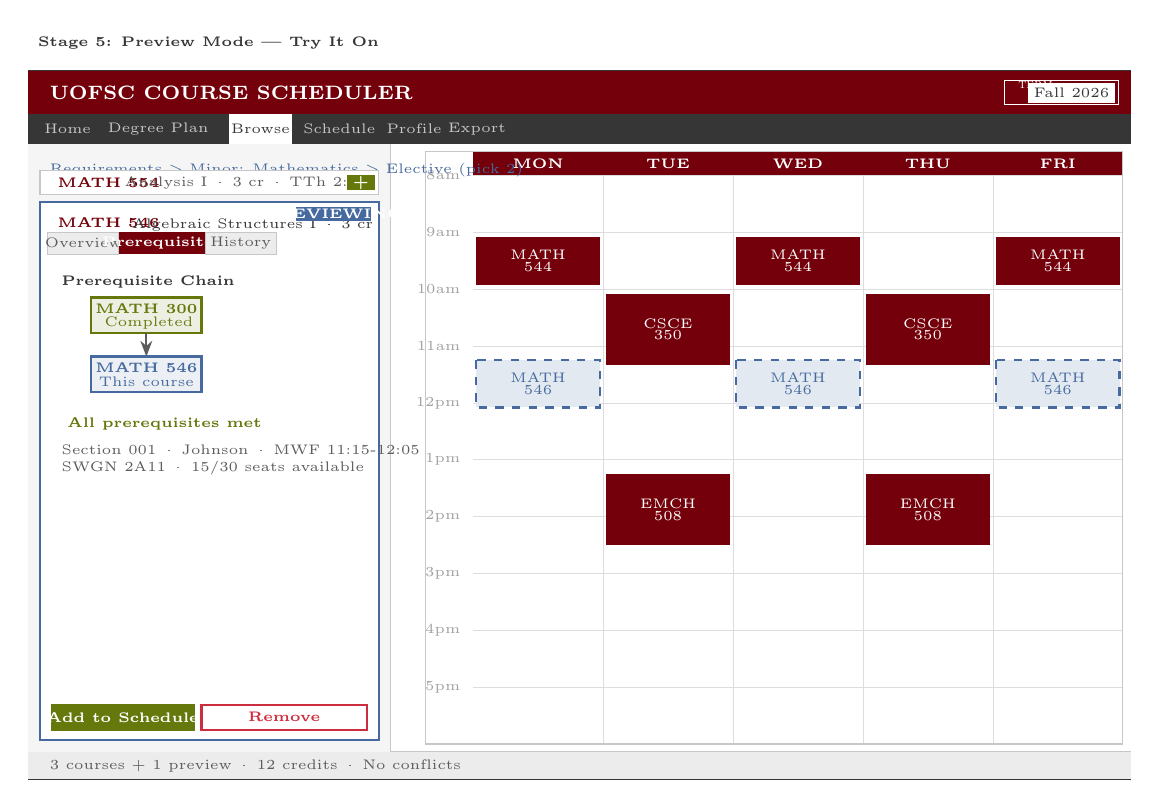
\begin{tikzpicture}
  \node[font=\fontsize{5.5}{6}\selectfont\bfseries,text=Black90,anchor=south west] at (0,\ph+0.15) {Stage 5: Preview Mode — Try It On};

  \draw[Black90,thin] (0,0) rectangle (\pw,\ph);
  \fill[white] (0,0) rectangle (\pw,\ph);

  \drawtopbar
  \drawnavbar{Browse}
  \drawstatusbar{3 courses + 1 preview \,·\, 12 credits \,·\, No conflicts}
  \drawleftpanel
  \drawschedulegrid

  \pgfmathsetmacro{\contenttop}{\ph-\tbh-\nbh-0.12}

  % Breadcrumb
  \node[font=\fontsize{3}{3.5}\selectfont,text=Atlantic,anchor=north west] at (0.15,\contenttop) {Requirements > Minor: Mathematics > Elective (pick 2)};

  % Compressed card above
  \pgfmathsetmacro{\compY}{\contenttop-0.22}
  \fill[white] (0.15,\compY) rectangle (\lw-0.15,\compY-0.3);
  \draw[Black30] (0.15,\compY) rectangle (\lw-0.15,\compY-0.3);
  \node[font=\fontsize{3}{3.5}\selectfont\bfseries,text=Garnet,anchor=west] at (0.25,\compY-0.15) {MATH 554};
  \node[font=\fontsize{2.8}{3}\selectfont,text=Black70,anchor=west] at (1.1,\compY-0.15) {Analysis I \,·\, 3 cr \,·\, TTh 2:50};
  \fill[Horseshoe] (\lw-0.55,\compY-0.05) rectangle (\lw-0.2,\compY-0.25);
  \node[font=\fontsize{4}{5}\selectfont\bfseries,text=white] at (\lw-0.375,\compY-0.15) {+};

  % ── EXPANDED DETAIL CARD: MATH 546 (Prerequisites tab) ──
  \pgfmathsetmacro{\expTop}{\compY-0.4}
  \pgfmathsetmacro{\expBot}{\sbh+0.15}
  \fill[white] (0.15,\expTop) rectangle (\lw-0.15,\expBot);
  \draw[Atlantic,thick] (0.15,\expTop) rectangle (\lw-0.15,\expBot);

  % Course title
  \node[font=\fontsize{4}{5}\selectfont\bfseries,text=Garnet,anchor=north west] at (0.25,\expTop-0.08) {MATH 546};
  \node[font=\fontsize{3.2}{4}\selectfont,text=Black90,anchor=north west] at (1.2,\expTop-0.09) {Algebraic Structures I \,·\, 3 cr};
  % "Previewing" badge
  \fill[Atlantic] (3.4,\expTop-0.06) rectangle (\lw-0.25,\expTop-0.24);
  \node[font=\fontsize{2.5}{3}\selectfont\bfseries,text=white] at ({(3.4+\lw-0.25)/2},\expTop-0.15) {PREVIEWING};

  % Tabs
  \pgfmathsetmacro{\tabY}{\expTop-0.38}
  \pgfmathsetmacro{\tabH}{0.28}
  \fill[Black10] (0.25,\tabY) rectangle (1.15,\tabY-\tabH);
  \draw[Black30] (0.25,\tabY) rectangle (1.15,\tabY-\tabH);
  \node[font=\fontsize{3}{3.5}\selectfont,text=Black70] at (0.7,\tabY-0.14) {Overview};
  % Prerequisites tab (active)
  \fill[Garnet] (1.15,\tabY) rectangle (2.25,\tabY-\tabH);
  \node[font=\fontsize{3}{3.5}\selectfont\bfseries,text=white] at (1.7,\tabY-0.14) {Prerequisites};
  % History tab (inactive)
  \fill[Black10] (2.25,\tabY) rectangle (3.15,\tabY-\tabH);
  \draw[Black30] (2.25,\tabY) rectangle (3.15,\tabY-\tabH);
  \node[font=\fontsize{3}{3.5}\selectfont,text=Black70] at (2.7,\tabY-0.14) {History};

  % Prerequisites content
  \pgfmathsetmacro{\preY}{\tabY-\tabH-0.15}
  \node[font=\fontsize{3.5}{4}\selectfont\bfseries,text=Black90,anchor=north west] at (0.3,\preY) {Prerequisite Chain};

  % Tree: MATH 300 -> MATH 546
  \pgfmathsetmacro{\treeY}{\preY-0.4}
  % MATH 300 node (completed = green)
  \fill[Horseshoe!12!white] (0.8,\treeY) rectangle (2.2,\treeY-0.45);
  \draw[Horseshoe,thick] (0.8,\treeY) rectangle (2.2,\treeY-0.45);
  \node[font=\fontsize{3.2}{4}\selectfont\bfseries,text=Horseshoe] at (1.5,\treeY-0.14) {MATH 300};
  \node[font=\fontsize{2.5}{3}\selectfont,text=Horseshoe] at (1.5,\treeY-0.32) {\checkmark\;Completed};

  % Arrow
  \draw[-{Stealth[length=2mm]},thick,Black70] (1.5,\treeY-0.45) -- (1.5,\treeY-0.75);

  % MATH 546 node (target)
  \pgfmathsetmacro{\targetY}{\treeY-0.75}
  \fill[Atlantic!10!white] (0.8,\targetY) rectangle (2.2,\targetY-0.45);
  \draw[Atlantic,thick] (0.8,\targetY) rectangle (2.2,\targetY-0.45);
  \node[font=\fontsize{3.2}{4}\selectfont\bfseries,text=Atlantic] at (1.5,\targetY-0.14) {MATH 546};
  \node[font=\fontsize{2.5}{3}\selectfont,text=Atlantic] at (1.5,\targetY-0.32) {This course};

  % Status message
  \pgfmathsetmacro{\msgY}{\targetY-0.65}
  \node[font=\fontsize{3.5}{4}\selectfont\bfseries,text=Horseshoe,anchor=north west] at (0.3,\msgY) {\checkmark\;All prerequisites met};

  % Section info
  \pgfmathsetmacro{\secY}{\msgY-0.35}
  \node[font=\fontsize{3}{3.5}\selectfont,text=Black70,anchor=north west] at (0.3,\secY) {Section 001 \,·\, Johnson \,·\, MWF 11:15-12:05};
  \node[font=\fontsize{3}{3.5}\selectfont,text=Black70,anchor=north west] at (0.3,\secY-0.2) {SWGN 2A11 \,·\, 15/30 seats available};

  % Action buttons
  \pgfmathsetmacro{\btnRowY}{\expBot+0.45}
  \fill[Horseshoe] (0.3,\btnRowY) rectangle (2.1,\btnRowY-0.32);
  \draw[Horseshoe,thick] (0.3,\btnRowY) rectangle (2.1,\btnRowY-0.32);
  \node[font=\fontsize{3.2}{4}\selectfont\bfseries,text=white] at (1.2,\btnRowY-0.16) {Add to Schedule};
  \fill[white] (2.2,\btnRowY) rectangle (\lw-0.3,\btnRowY-0.32);
  \draw[Rose,thick] (2.2,\btnRowY) rectangle (\lw-0.3,\btnRowY-0.32);
  \node[font=\fontsize{3}{3.5}\selectfont\bfseries,text=Rose] at ({(2.2+\lw-0.3)/2},\btnRowY-0.16) {Remove};

  % Schedule blocks — 3 solid + 1 preview (dashed blue)
  \drawcourseblock{1}{5.25}{6.5}{Garnet}{EMCH\\508}{solid}
  \drawcourseblock{3}{5.25}{6.5}{Garnet}{EMCH\\508}{solid}
  \drawcourseblock{0}{1.08}{1.92}{Garnet}{MATH\\544}{solid}
  \drawcourseblock{2}{1.08}{1.92}{Garnet}{MATH\\544}{solid}
  \drawcourseblock{4}{1.08}{1.92}{Garnet}{MATH\\544}{solid}
  \drawcourseblock{1}{2.08}{3.33}{Garnet}{CSCE\\350}{solid}
  \drawcourseblock{3}{2.08}{3.33}{Garnet}{CSCE\\350}{solid}

  % MATH 546 preview — MWF 11:15-12:05 (hours 3.25-4.08)
  \drawcourseblock{0}{3.25}{4.08}{Atlantic}{MATH\\546}{dashed}
  \drawcourseblock{2}{3.25}{4.08}{Atlantic}{MATH\\546}{dashed}
  \drawcourseblock{4}{3.25}{4.08}{Atlantic}{MATH\\546}{dashed}
\end{tikzpicture}

\end{document}
